%!TEX root = ../dissertation.tex
% this file is called up by thesis.tex
% content in this file will be fed into the main document

\graphicspath{{7-timbre/figures/}}

\chapter{Synthesizer-Aided Multi-Instrument Transcription}
\label{ch:timbre}

In Chapter \ref{ch:introduction}, we introduced the idea of extending a music transcription model with an additional synthesizer component that can convert the transcribed information back to the input audio, forming an analysis/synthesis framework as depicted in the encoder-decoder architecture in Figure \ref{fig:autoencoder}.
By doing so, we anticipated that the two components --- the transcriber and the synthesizer --- can work together to better translate information between the two representations, i.e. audio waveform and the transcribed semantic information of the music.
One motivation for employing such analysis/synthesis framework is that the advent of many successful deep learning techniques and the improved hardware capability may allow us to convert an audio signal completely into the constituent pieces of musical information that we want to transcribe, that are entangled in an extremely sophisticated way in the audio signal.
In the preceding chapters, we have considered deep learning solutions to various problems in music analysis and synthesis, such as monophonic pitch tracking (Chapter \ref{ch:monophonic}), music synthesis with controllable timbre (Chapter \ref{ch:synthesis}), and polyphonic music transcription (Chapter \ref{ch:adversarial}).
These problems correspond to a certain subset of the full encoder-decoder architecture, and in each chapter we discussed how the design choices in the model architecture and dataset construction affect the experimental results and the real-world applicability.

Having learned the lessons from these, in this chapter we aim to construct an automatic music transcription system that encompasses the full analysis/synthesis cycle, by considering the general problem of multi-instrument polyphonic music transcription.
We propose an autoencoder architecture that appends a synthesis model on top of a transcription model, and we verify the effects of the appended synthesizer in the experiments.
As in Chapter \ref{ch:synthesis}, the synthesizer component is capable of capturing the different aspects of various timbres in the dataset using a learned timbre space representation.
We show that the synthesizer component can serve as a regularizer to the transcriber, providing a form of prior knowledge on the spectral and temporal characteristics of the timbres. 
% \TODO{some conclusive sentence summarizing the results of this chapter}

\section{Introduction}

Multi-instrument music transcription aims to extract not only the occurrences of multiple simultaneous pitches and notes but also the types of one or more instruments corresponding to those notes.
Since it poses additional challenges to the already difficult problem of polyphonic music transcription, studies on the complete multi-instrument polyphonic transcription problem are relatively rare.
Instead, most studies on analyzing multi-instrument audio focus on either developing a discriminative model for polyphonic where timbre information is disregarded~\cite{bittner2017deepsalience} %\TODO{cite more}
or the problem of instrument recognition, while not identifying the individual notes that belongs to the recognized instruments~\cite{lostanlen2016spiral}. %\TODO{cite more}
To take both polyphonic notes and multiple instruments into account, a model has to carefully incorporate the prior knowledge of how pitch and timbre are reflected in the audio signal, e.g. using a probabilistic latent component model~\cite{benetos2015probabilistic} or a variant of non-negative matrix factorization~\cite{grindlay2009eigeninstruments}.
To produce outputs in multiple domains, these models have to include an intricate set of design choices to implement a mathematical representation of the prior knowledge.

Meanwhile, the main premise of deep learning is quite opposite of how those models are designed.
Rather than writing down the set of rules manually, layers of simple calculations can serve as a very effective function approximator, that can produce just about anything when an enough amount of data is fed to the black box.
In these models, the prior knowledge baked into the model architecture is minimal.
Take the Onsets and Frames model~\cite{hawthorne2018onsetsframes} for example; the model output has 88 dimensions corresponding to each key of the piano, but the 88 keys are treated as a separate multi-label target, without utilizing the knowledge that each key should represent a certain frequency that the quasi-periodic signal in the input follows.
Because of this lack of ``inductive bias'', deep learning models typically have to be trained with a very large amount of data; in other words, they are less sample efficient.


Generative models for transcription, such as a Bayesian network representation of spectrogram~\cite{bergkirkpatrick2014unsupervised}, takes the opposite approach.
These models define the process of generating sound entirely from the parameterized sources that typically convey a physical interpretation, such as the modeling of attack-decay-sustain-release (ADSR) curves or the energy distribution along harmonics. 
Compared to data-driven models with a lot of learnable parameters, however, those interpretable transcription models often lack the flexibility to be applicable for a wider variety of inputs.

In this chapter, we explore the possibility of finding a compromise between the two extremes.
Specifically, we examine how to induce the transcription model to make predictions such that, when synthesized back into audio, resemble the original audio input.
We do this by appending a neural music synthesis model to the transcription model, and the synthesis model is specifically designed to describe the sound generation process with a small number of interpretable parameters, which is restrictive enough to guide the transcription model to more accurate predictions, yet flexible enough to be learnable in a data-driven manner.
We evaluate this approach with a multi-instrument transcription task and show that a synthesis model can serve as an effective regularizer. % \TODO{describe qualitative improvement}

\section{Background}


\subsection{Multi-Instrument Music Transcription}

\cite{itoyama2011bayesian}: instrument recognition, \TODO{add more; interconnected with source separation}

\cite{grindlay2009eigeninstruments}: Hierarchical eigeninstruments

\cite{benetos2015probabilistic}: Probabilistic model (PLCA), spectral template, EM maximization

\cite{thickstun2017musicnet}: MusicNet, \cite{thickstun2018invariances} invariances,

\subsection{Deep Clustering}

\cite{hershey2016deepclustering}

\subsection{Source-Filter Synthesis}

\cite{heittola2009separation} (instrument recognition)

\subsection{Synthesizer Component for Transcription}

\citeA{li2017infinite} explored the idea of using on-the-fly synthesized training dataset for piano transcription, using a simple fully-connected neural network operating on the CQT representation.
The idea of using generative models to predict multiple fundamental frequencies is also not new \cite{dubois2005harmonic,cemgil2006generative}, but the authors relied on manually designed generative models for sound generation, which limits the expressibility and the generalizability of the model.
Using deep generative models can be a direction for overcoming these limitations, since the recent neural network approaches for audio generation are capable of producing highly realistic sounds.

\cite{choi2019drum} \cite{bergkirkpatrick2014unsupervised}


\section{Method}

We first describe the synthesizer model, followed by the modifications to the Onsets and Frames~\cite{hawthorne2018onsetsframes} transcription model made to allow the concatenation of the two models.

\subsection{Synthesizer Model}

The synthesizer model takes a per-instrument piano roll representation of symbolic music (see Figure \ref{fig:transcription-to-piano-rolls}) and uses a learned instrument embedding to predict the Mel spectrogram of the corresponding audio.
We are assuming here that predicting Mel spectrograms is equivalent to synthesizing the audio for our purposes, since we have seen in Chapter \ref{ch:synthesis} that Mel spectrograms contain most of the perceivable information present in the audio content, and the original audio can readily be reconstructed using sample-based synthesis models like WaveNet~\cite{oord2016wavenet}.

The synthesizer consists of two subcomponents, the envelope estimator and the waveshaper, respectively implementing the temporal and spectral characteristics of the sound being synthesized.
The computation in each subcomponent is performed independently for each pitch-instrument combinations, and their results are combined to obtain the resulting Mel spectrogram, as shown in Figure \ref{fig:synthesizer-architecture}.
Both components take the instrument embedding in order for the synthesized audio to exhibit different temporal and spectral behaviors depending on the instrument, and together they ensure that the synthesis model only creates harmonic sounds with the frequency corresponding to the pitch of input notes and the spectral envelope consistent among each instrument.

The envelope estimator component predicts the temporal envelope of each note, by mapping the note activities into a latent space using a one-dimensional convolution layer, followed by a FiLM layer~\cite{perez2018film} to condition on the instrument.
A GRU layer~\cite{cho2014seq2seq} is then applied in order to model the temporal behavior, such as the attack-decay-sustain-release (ADSR) curves.
Meanwhile, the waveshaper component performs a subtractive synthesis to obtain the spectrum corresponding to each pitch and instrument.
We use two types of source waves, sawtooth and triangular, to make it easily adaptable to the timbres that primarily consists of odd harmonics, such as the clarinet.
The instrument embedding is used to predict the transfer function in the Mel frequency domain to be applied to each source spectrum, which is modeled as a polynomial function mapping Mel frequencies to log magnitudes.
The Mel spectrogram corresponding to each note can then be calculated in the complex domain, by assigning a random initial phase to each pitch-instrument pair and multiplying the temporal envelope predicted by the envelope estimator.
All of the per-note Mel spectrograms are then added to obtain the final Mel spectrogram output.



\begin{figure}
	\centering
	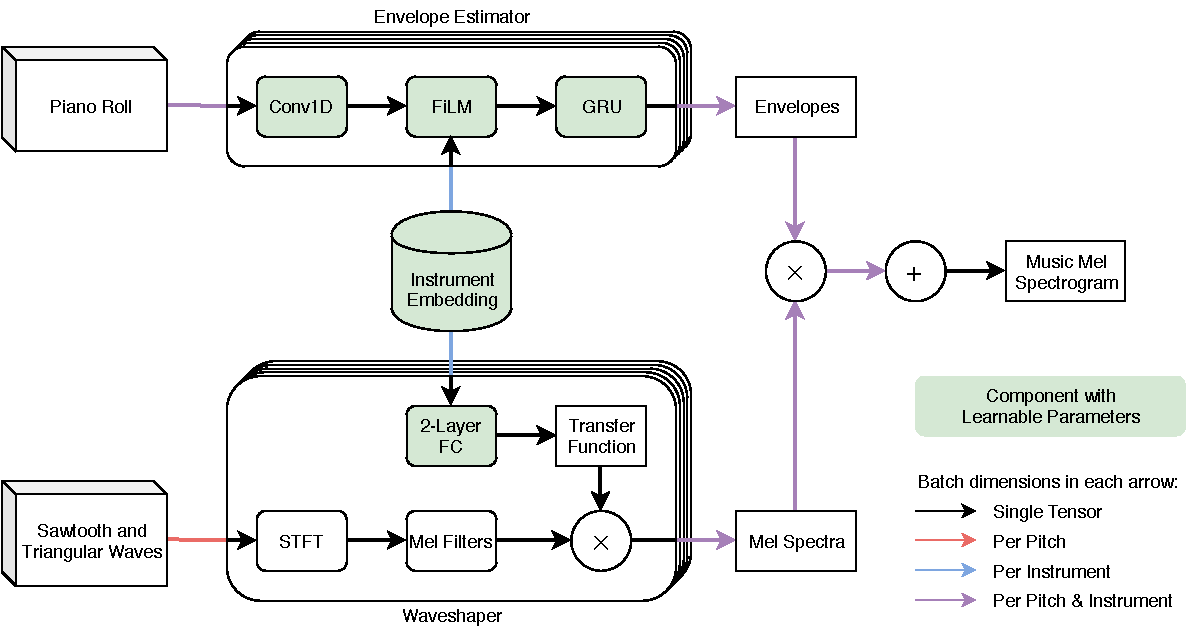
\includegraphics[width=\textwidth]{synthesizer-architecture.pdf}
	\caption{The synthesizer architecture. The temporal and spectral characteristics of each notes are respectively modeled by the envelope estimator and the waveshaper. This structure enforces each instrument to have consistent spectral and temporal envelopes across the pitch.}\label{fig:synthesizer-architecture}
\end{figure}


\subsection{Training Transcriber with Appended Synthesizer}

To append the synthesizer component to the output of the transcription model while keeping the full model differentiable, we expand the fully-connected layer predicting the frame activation to additionally predict the instrument embedding corresponding to each time-frequency bin.
Using the expanded outputs, the frame activations and the predicted embedding can be fed to the synthesizer component.
The frame activations are binarized before feeding to the synthesizer, and we use a gradient-stop for this connection.

The synthesizer model is separately trained, and the transcriber model is then optimized to minimize the sum of three losses:
\begin{equation}
\mathcal{L}_{\text{Overall}} = \mathcal{L}_{\text{Onsets \& Frames}} + \lambda \left ( \mathcal{L}_{\text{Embedding}} + \mathcal{L}_{\text{Synthesizer}} \right )
\end{equation}
The first term, $\mathcal{L}_{\text{Onsets \& Frames}}$, is the loss of the Onsets and Frames model which is the sum of the binary cross entropy of the onsets, offsets, and frame predictions.
We define $\mathcal{L}_{\text{Embedding}}$ as the mean squared error (MSE) between the predicted instrument embedding and the ground truth, and $\mathcal{L}_{\text{Synthesizer}}$ is defined as the mean cosine distance between the predicted and the ground-truth Mel spectra:
\begin{equation}
\mathcal{L}_{\text{Synthesizer}} = \mathbb{E}_{\hat{\mathbf{s}}, \mathbf{s}} \left [ 1 - \frac{ \hat{\mathbf{s}} \cdot \mathbf{s} }{\lVert \hat{\mathbf{s}} \rVert \lVert \mathbf{s} \rVert} \right ]
\end{equation}
where $\mathbf{s}$ follows the distribution of Mel spectra in the input audio, and $\hat{\mathbf{s}}$ is the Mel spectra predicted by the synthesizer based on the transcription predicted from $\mathbf{s}$.

\section{Experimental Setup}

We use the MusicNet dataset~\cite{thickstun2017musicnet} to train both the synthesizer and the transcriber.
The dataset contains 2,048 minutes of classical chamber music audio and labels, which comprises 330 recordings of various ensembles.
The dataset contains annotations of 11 General MIDI instruments: Acoustic Grand Piano, Harpsichord, Violin, Viola, Cello, Contrabass, French Horn, Oboe, Bassoon, Clarinet, and Flute.
Different recordings in the dataset have drastically different tuning, ranging more than a semitone in some recordings which would result in a wrong transcription even by a perfect transcriber.
To alleviate this, we preprocess the dataset by running a tuning estimator implemented in librosa~\cite{mcfee2015librosa} on each track and pitch-shifted any recordings that are more than 20 cents apart from the A440 tuning.

Unlike in Chapter~\ref{ch:adversarial}, we use the original Onsets and Frames model size of 512, and the transcription model contains 10 million parameters.
We use a 2-dimensional instrument embedding space to represent the distribution of the 11 instruments, and the polynomial transfer functions used in the subtractive synthesis are modeled by cubic B\'{e}zier curves.


The audio is resampled to 16kHz, and a training batch is composed of eight 20-second audio segments and labels.
We use Adam optimizer~\cite{kingma2015adam} with learning rate 0.0006, and the learning rate decay of factor 0.98 is applied every 1000 steps.
We ran the optimization for 180,000 steps and report the transcription accuracy evaluated on the 10 test recordings provided in the MusicNet dataset.

\section{Results}

\subsection{Synthesizer Output}

\subsection{Transcription Accuracy}

\subsection{Multi-Instrument Transcription}

\begin{itemize}
	\item Trained Synthesizer
	\item Transcription Metrics
	\item Multi-instrument
\end{itemize}

\subsection{MusicNet Inspector}



\section{Conclusion}

\begin{itemize}
	\item Discussion points: unison, dot product space, Lipschitz; volume information
\end{itemize}

